\section{Data Combination}
Once all files have been downloaded, the user should the Data Combination tab. In this view, it can be selected a Measure ID from the options available (\Cref{fig:DataCombination}). All measure IDs shown in downloaded files my be not available, since the list of measure IDs is filtered depending on the data contained. Measure IDs containing files with code 007 will not be added to the list, since these  measurements will not contain all the data needed for the analysis.
\begin{figure}[H]
\centering
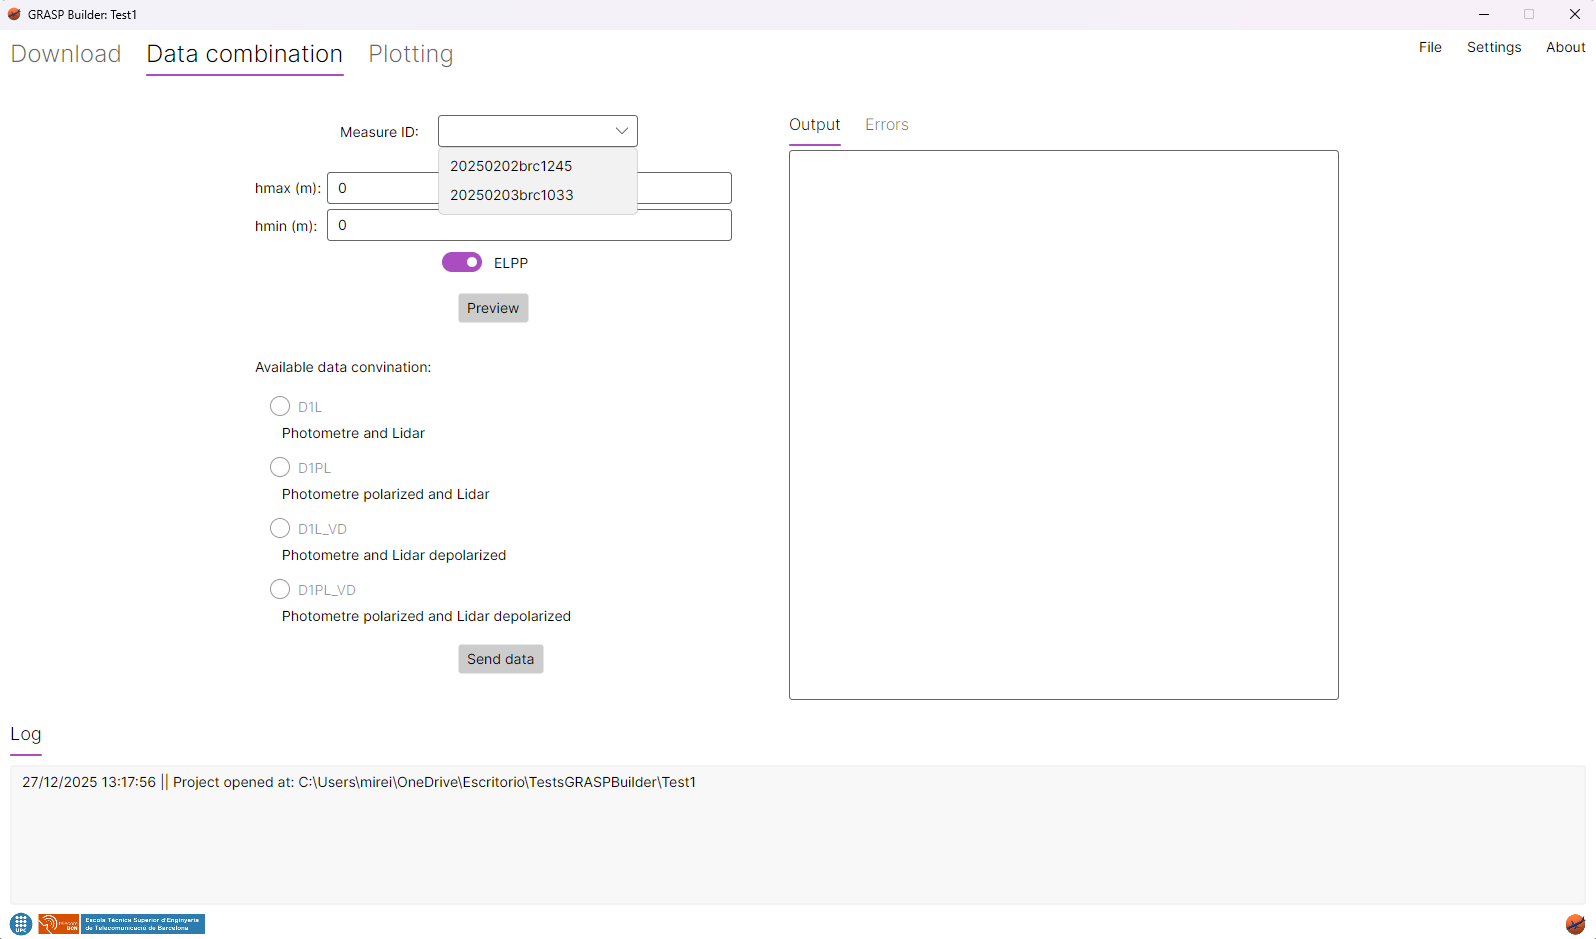
\includegraphics[width=16cm]{img/DataCombination.png}
\caption[Data combination view]{\footnotesize{Data combination view}}
\label{fig:DataCombination}
\end{figure}
When a Measure ID is selected, the GetHeights script is executed, so the minimum and maximum height can be retrieved instead of having 0 values. The, the Preview script has to be launched in order to preview the data and obtain the available configuration options. This script can be launched manually using the "Preview" button all the desired times with the two different type of data (ELPP and VD, if possible). 
Default configured data type to show is ELPP, since this data is always available (\Cref{fig:SelectMeasureID_ELPP}). The other option is VD (\Cref{fig:SelectMeasureID_VD}).
\begin{figure}[H]
\centering
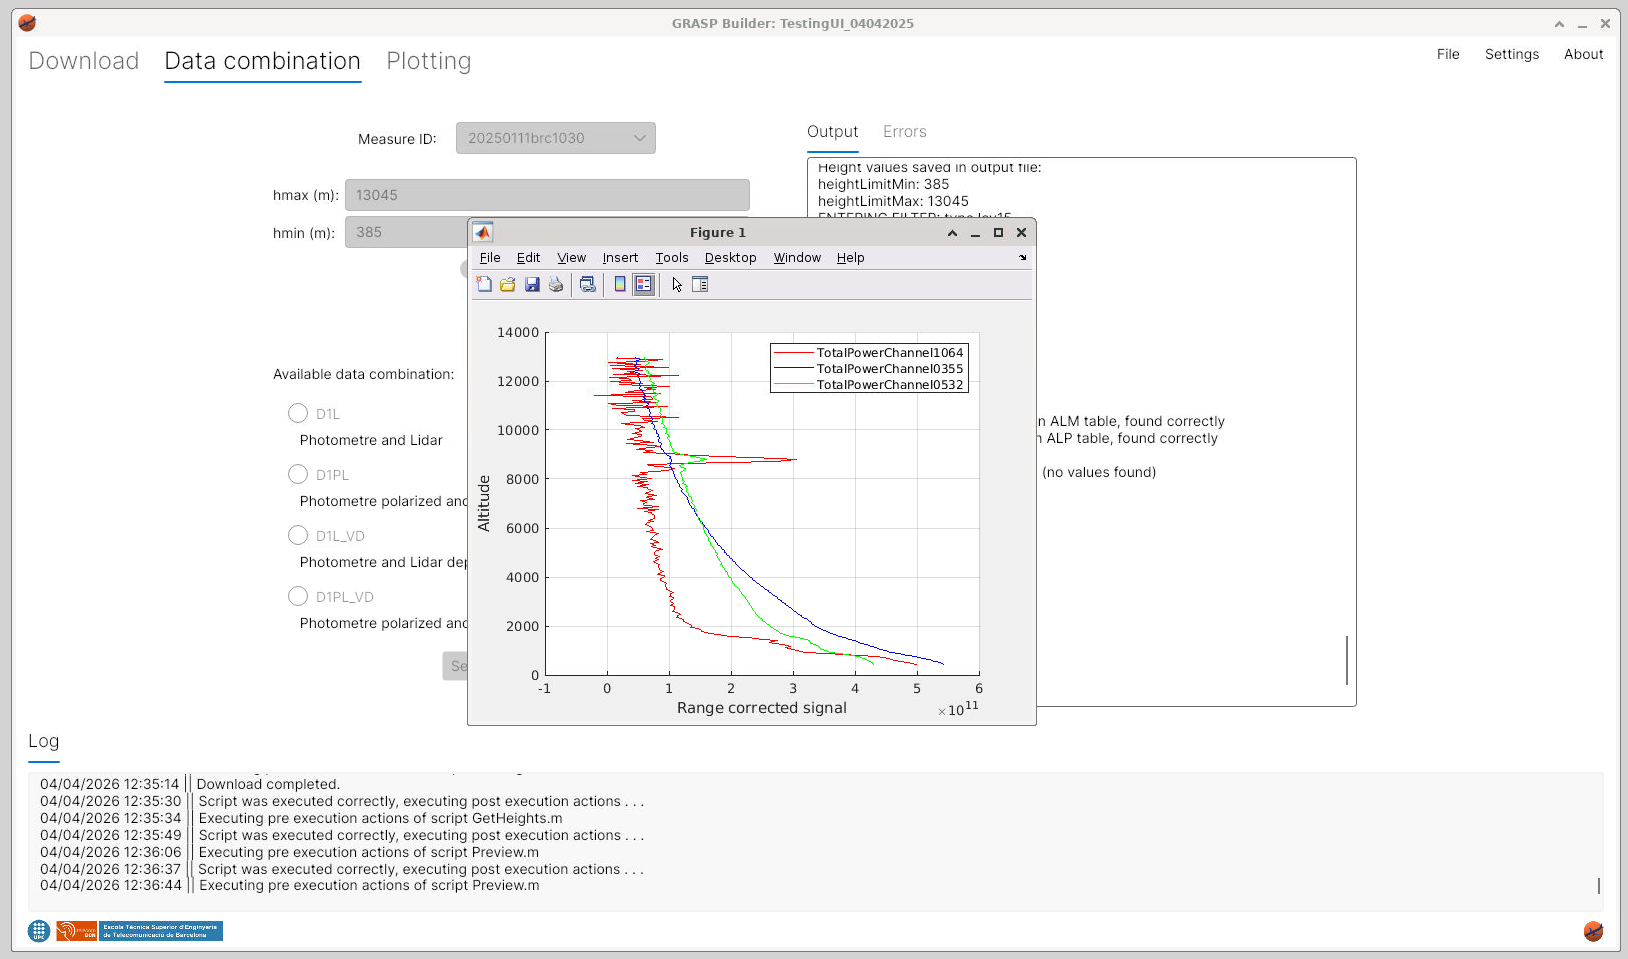
\includegraphics[width=16cm]{img/SelectMeasureID_ELPP.png}
\caption[Execute preview with ELPP option]{\footnotesize{Execute preview with ELPP option}}
\label{fig:SelectMeasureID_ELPP}
\end{figure}
During the script execution, the previsualitzatin figure will be shown. In order to update the application with the available configurations, the Matalb figure needs to be closed, in order to execute the corresponding script post execution actions.
\begin{figure}[H]
\centering
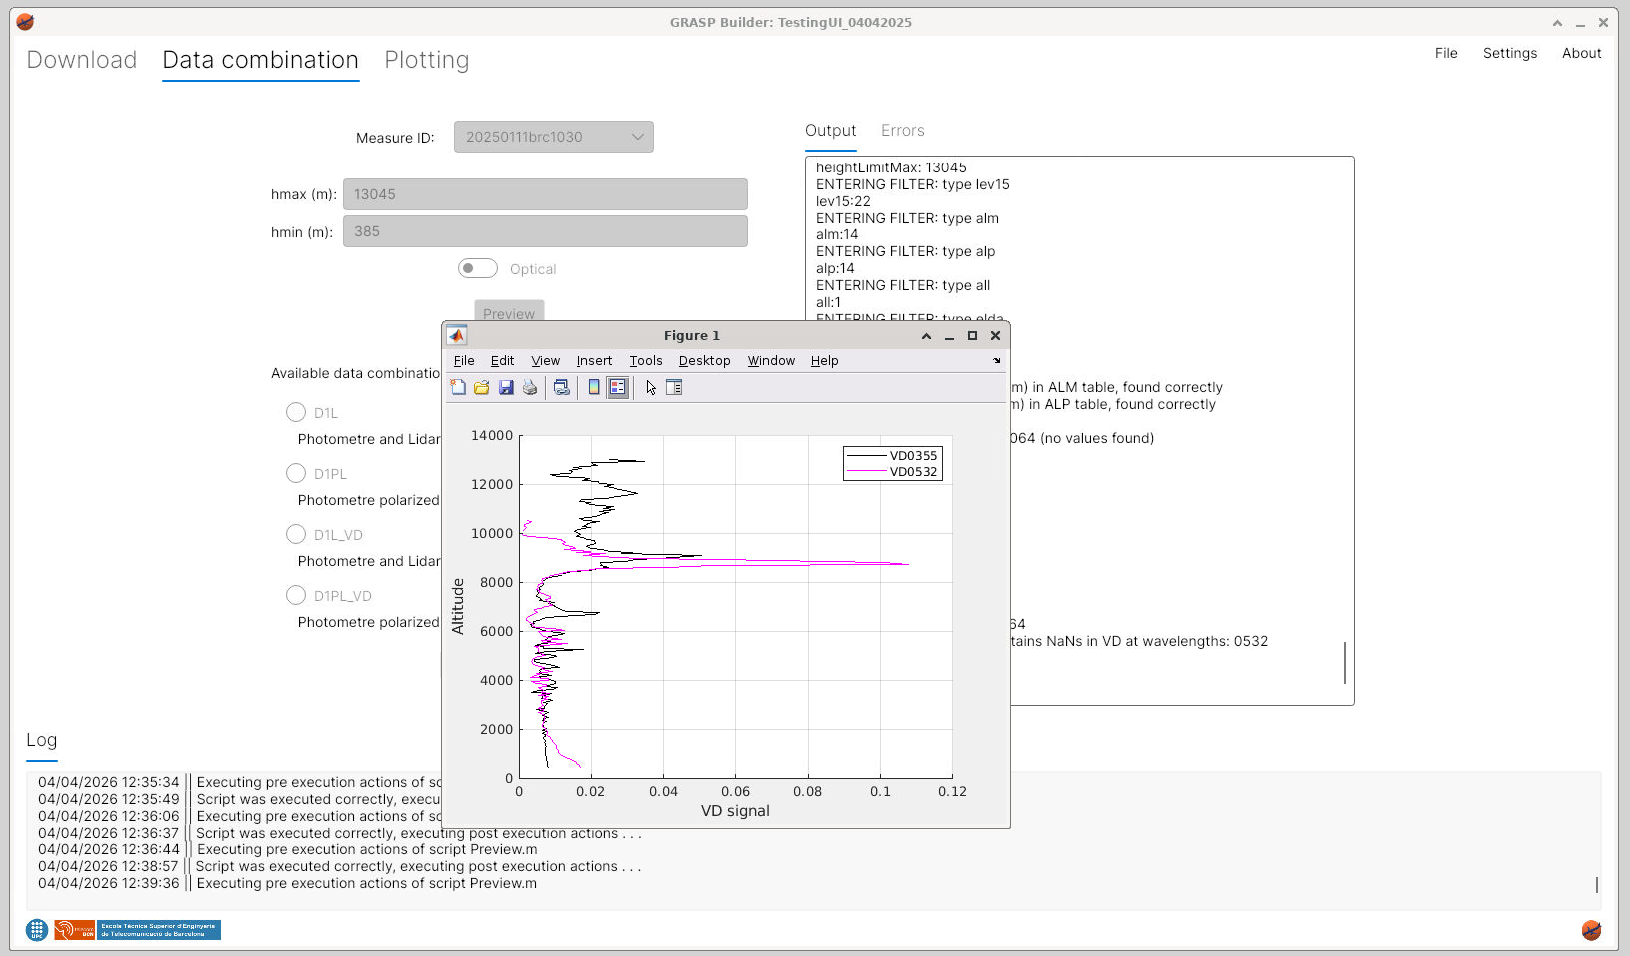
\includegraphics[width=16cm]{img/SelectMeasureID_VD.png}
\caption[Execute preview with VD option and heighs defined]{\footnotesize{Execute preview with VD option and heighs defined}}
\label{fig:SelectMeasureID_VD}
\end{figure}
It is recommended to review the height values before starting the data combination process, since NaN values must be avoided in order to run the algorithm successfully.\smallskip\\
\Cref{fig:SelectMeasureID_VD_heights} shows and example of the preview window with the heights defined and Optical data selected.
\begin{figure}[H]
\centering
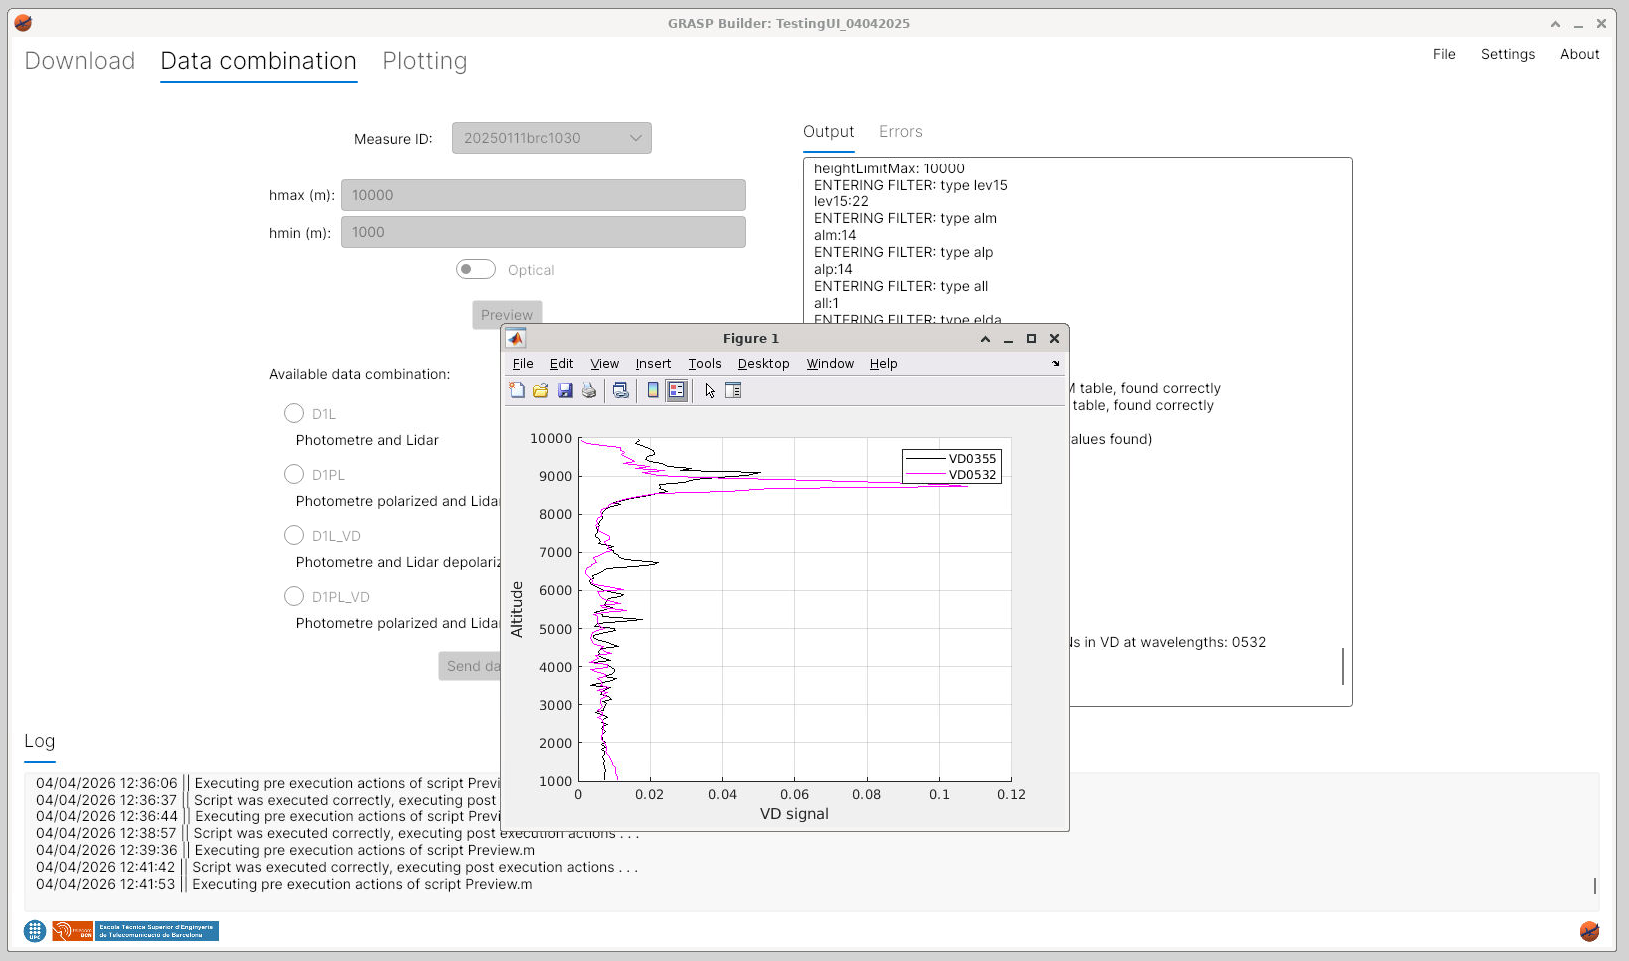
\includegraphics[width=16cm]{img/SelectMeasureID_VD_heights.png}
\caption[Execute preview with VD option]{\footnotesize{Execute preview with VD option}}
\label{fig:SelectMeasureID_VD_heights}
\end{figure}
Every time a script in this window is executed, all buttons will be disabled, and once the plot window is closed, GUI elements will be updated and enabled again.\smallskip\\
When a configuration is selected, by clicking the "Send ata" button, the SendFiles script is executed. If the script is executed successfully and .sdat file has been written successfully, .yml configuration file will be automatically created and GRASP algorithm will be executed.
\begin{figure}[H]
\centering
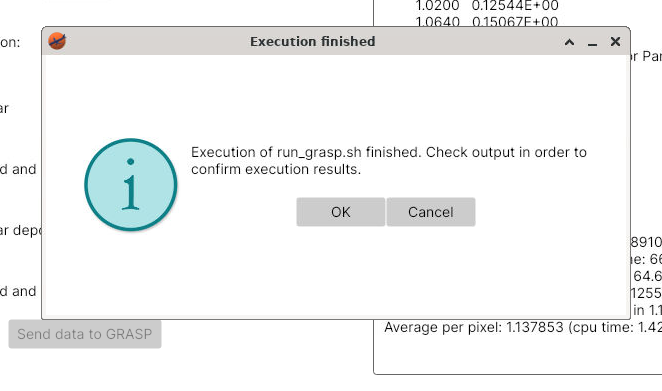
\includegraphics[width=12cm]{img/InforGRASPFinished.png}
\caption[Execute SendFiles script]{\footnotesize{Execute SendFiles script}}
\label{fig:InfoGRASPFinished}
\end{figure}
{Once GRASP has finished executing, it will appear an information message notifying the user \Cref{fig:InfoGRASPFinished}. If something went wrong, an error will appear.}